\documentclass[xcolor=table]{beamer}

\usepackage{amsmath}
\usepackage{amssymb}
\usepackage[utf8]{inputenc}

\usepackage{hyperref}

\usepackage{amssymb} %for Lagrangian L, order O

%\usepackage{gensymb}
\usepackage{siunitx}
\usepackage{xcolor}
\usepackage{colortbl}
\usepackage{cancel}
\usepackage[normalem]{ulem}
\usepackage{calc}
\usepackage{ragged2e}

%for side-by-side figures
\usepackage{graphicx}
\usepackage[compatibility=false]{caption}

\setlength{\parindent}{2em}
\setlength{\parskip}{1em}
\renewcommand{\baselinestretch}{1.1}
\setlength\parindent{0pt} % Removes all indentation from paragraphs - comment this line for an assignment with lots of text

\usetheme{Madrid}

\definecolor{green}{HTML}{C4E76D}
\definecolor{red}{HTML}{F57F73}
\definecolor{yellow}{HTML}{F5E274}

%----------------------------------------------------------------------------------------
%	TITLE SECTION
%----------------------------------------------------------------------------------------
\title[Observation of the W (1983)] %optional
{Experimental observation of isolated large transverse energy electrons with associated missing energy at $\sqrt{s}=\SI{540}{GeV}$}
 
\subtitle{}
 
\author[Braden Moore] % (optional, for multiple authors)
{Braden~Moore}
 
\institute[] % (optional)
{
  School of Physics\\
  The University of Melbourne\\
  \vspace{0.5cm}
}
 
\date[11 March 2016] % (optional)
{Advanced Seminar, 11 March 2016}
 
\logo{
\includegraphics[height=1.5cm]{images/university-of-melbourne-logo.jpg}}

%\setbeamerfont{caption}{size=\footnotesize}

%----------------------------------------------------------------------------------------
\begin{document}
 
\frame{\titlepage}

%------------------------------

\begin{frame}
\frametitle{Overview of the paper}
\fontsize{9pt}{12}\selectfont


\begin{itemize}
\item $p\bar{p}\to e\nu$ events previously predicted to be mediated by $W$ boson, as in:
\begin{equation*}
p\bar{p}\to W^{\pm}\to e^{\pm}+\nu
\end{equation*}
\item $p\bar{p}$ collision events at UA1 in the SPS at CERN investigated for $p\bar{p}\to e\nu$
\item 6 events with high-energy electrons and a neutrino of equal and opposite transverse momenta found in $\SI{18}{nb^{-1}}$ data set; suggests two body decay $W\to e\nu$
\item mass of $W$ is determined experimentally as 
\begin{equation*}
m_W=\left(81^{+5}_{-5}\right)\text{GeV}/\text{c}^2
\end{equation*}
\item experimental mass and cross-section found to be in excellent agreement with Weinberg-Salam predictions
\end{itemize}


\end{frame}

%------------------------------s

\begin{frame}
\frametitle{Particle physics up to 1983}
\fontsize{9pt}{12}\selectfont

\begin{itemize}
\item 1897 - electron discovered
\item 1932 - positron discovered
\item 1937 - muon discovered
\item 1956 - (electron) neutrino discovered
\item 1962 - muon neutrino discovered
\item 1968 - Glashow, Weinberg and Salam formulate unified electroweak theory
\item 1969 - partons observed
\item 1975 - tau discovered
\item 1983 - ???
\end{itemize}


\end{frame}
%------------------------------

\begin{frame}
\frametitle{Particle physics up to 1983}
\fontsize{9pt}{12}\selectfont

\begin{itemize}
\item 1897 - electron discovered
\item 1932 - positron discovered
\item 1937 - muon discovered
\item 1956 - (electron) neutrino discovered
\item 1962 - muon neutrino discovered
\item 1968 - Glashow, Weinberg and Salam formulate unified electroweak theory
\item 1969 - partons observed
\item 1975 - tau discovered
\item 1983 - W and Z bosons discovered
\end{itemize}


\end{frame}
%------------------------------


\begin{frame}
\frametitle{Predictions of W mass + cross-section}
\fontsize{11pt}{10}\selectfont


\begin{equation*}
m_{W}=(82\pm 2.4)~\SI{}{GeV/c^2}
\end{equation*}

\begin{equation*}
\sigma(p\bar{p}\to W^{\pm}\to e^{\pm}+\nu)\simeq 0.4\times 10^{-33} k ~\SI{}{cm^2}= 0.4k~\SI{}{nb}
\end{equation*}

\begin{itemize}
\item $k$ is an enhancement factor of $\sim 1.5$
\item in $\SI{18}{nb^{-1}}$ sample, would expect $\sim 18\times 0.4k=7.2k$ events
\end{itemize}


\end{frame}


%------------------------------


\begin{frame}
\frametitle{Super Proton Synchrotron (SPS) @ CERN}
\fontsize{7pt}{12}\selectfont

\begin{columns}

\column{0.5\linewidth}

\begin{figure}[h]
\centering
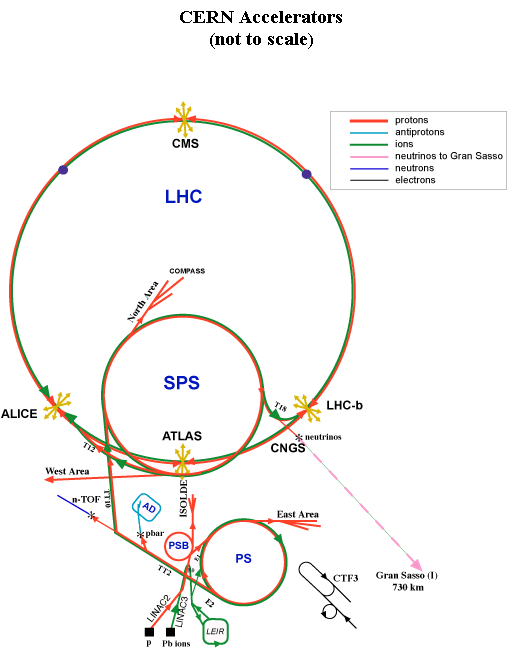
\includegraphics[height=0.8\textheight]{images/sps.png}
\end{figure} 

\column{0.5\linewidth}
\begin{itemize}
\item 1957 - Synchrocyclotron starts up
\item 1959 - Proton Synchrotron starts up
\item 1976 - Super Proton Synchrotron starts up
\item 1989 - LEP first injection
\item 1999 - Antiproton Decelerator approved
\item 2000 - LEP final shutdown
\item 2008 - LHC starts up
\end{itemize}

\end{columns}


\end{frame}

%------------------------------

\begin{frame}
\frametitle{Underground Area 1 (UA1) - detector}
\fontsize{9pt}{12}\selectfont

\begin{figure}[h]
\centering
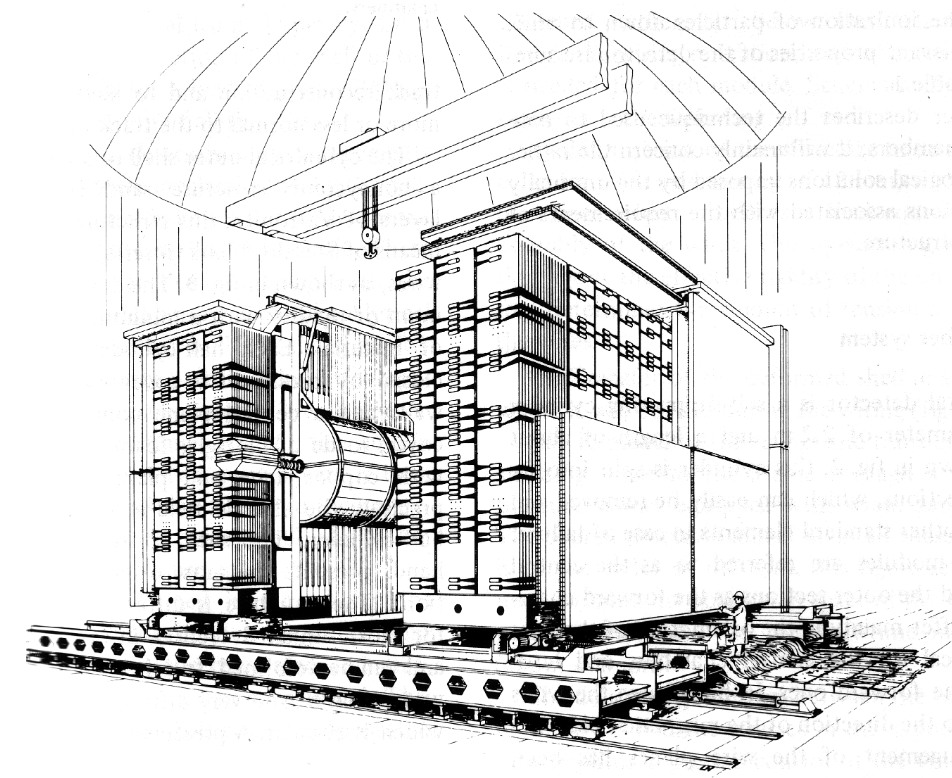
\includegraphics[height=0.75\textheight]{images/ua1-overview.png}
\end{figure}

\end{frame}

%------------------------------

\begin{frame}
\frametitle{Underground Area 1 (UA1) - detector}
\fontsize{9pt}{12}\selectfont

\begin{figure}[h]
\centering
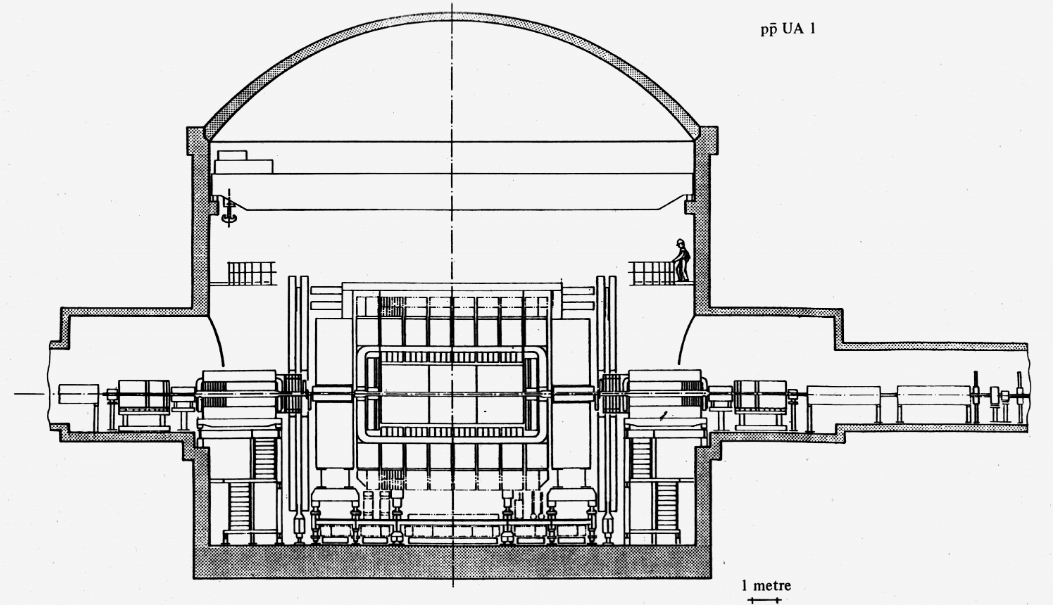
\includegraphics[height=0.7\textheight]{images/ua1-sideview.png}
\end{figure}

\end{frame}

%------------------------------

\begin{frame}
\frametitle{Underground Area 1 (UA1) - detector}
\fontsize{12pt}{12}\selectfont

\begin{itemize}
\item ran from 1981 until 1990
\item moveable detector (see also UA2) custom built around SPS for $p\bar{p}$ collisions
\item could be rolled back to allow fixed-target operation of SPS
\end{itemize}



\end{frame}

%------------------------------

\begin{frame}
\frametitle{Underground Area 1 (UA1) - detector}
\fontsize{9pt}{12}\selectfont

\begin{itemize}
\item transverse dipole magnet produced uniform field of 0.7T over $7\times 3.5\times 3.5\si{m^3}$
\item central detector = six-chambered cylinder, $\SI{5.8}{m}$ length, $\SI{2.3}{m}$ diameter
\item produced bubble-chamber quality pictures of each interaction
\end{itemize}

\begin{figure}[h]
\centering
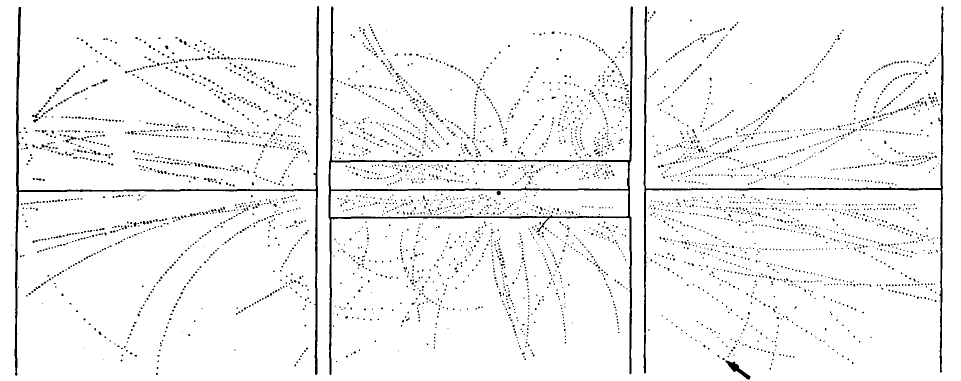
\includegraphics[width=0.85\textwidth]{images/track-imaging.png}
\end{figure}


\end{frame}

%------------------------------
\begin{frame}
\frametitle{Underground Area 1 (UA1) - detector}
\fontsize{9pt}{12}\selectfont

\begin{columns}

\column{0.5\linewidth}
\begin{itemize}
\item 48 barrel EM calorimeters, called `gondolas'
\end{itemize}

\begin{figure}[h]
\centering
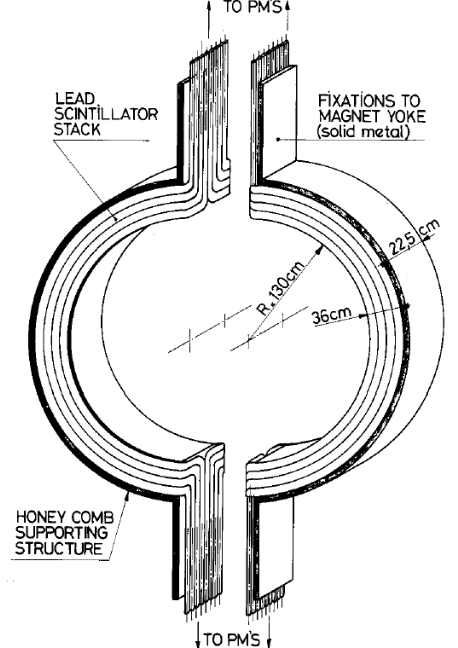
\includegraphics[height=0.65\textheight]{images/gondola.png}
\end{figure}

\column{0.5\linewidth}
\begin{itemize}
\item 64 end-cap EM calorimeters, called `bouchons'
\end{itemize}
\begin{figure}[h]
\centering
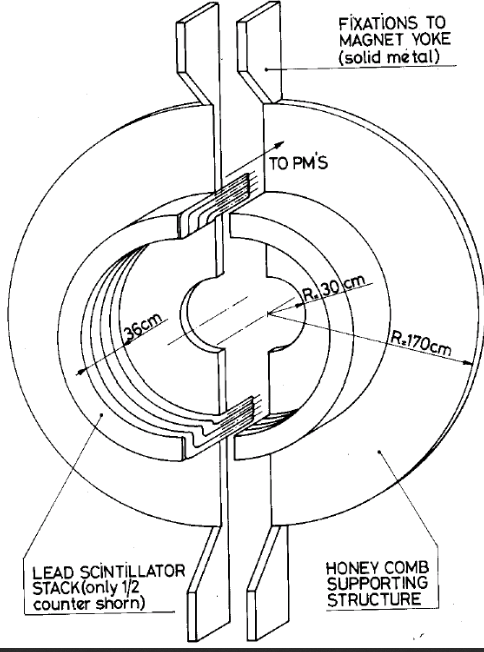
\includegraphics[height=0.65\textheight]{images/bouchon.png}
\end{figure}

\end{columns}

\end{frame}
%------------------------------

\begin{frame}
\frametitle{Underground Area 1 (UA1) - detector}
\fontsize{9pt}{12}\selectfont


\begin{itemize}
\item transverse energy $E_T$ a very important variable; attenuation length of scintillators in calorimeter are arranged to match variation over $\sin\theta$
\item from this $E_T=E\sin\theta$ can be directly measured
\end{itemize}

\begin{figure}[h]
\centering
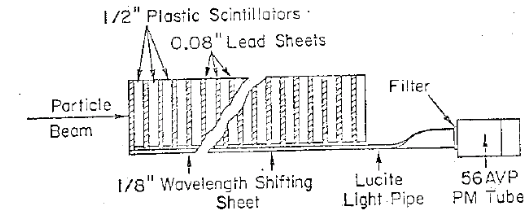
\includegraphics[width=0.8\textwidth]{images/gondola-scintillators.png}
\end{figure}


\end{frame}
%------------------------------

\begin{frame}
\frametitle{Electron/hadron separation}
\fontsize{9pt}{12}\selectfont


\begin{itemize}
\item electromagnetic showers identifed by characteristic transition curve
\item 90\% of electrons are detected
\end{itemize}

\begin{figure}[h]
\centering
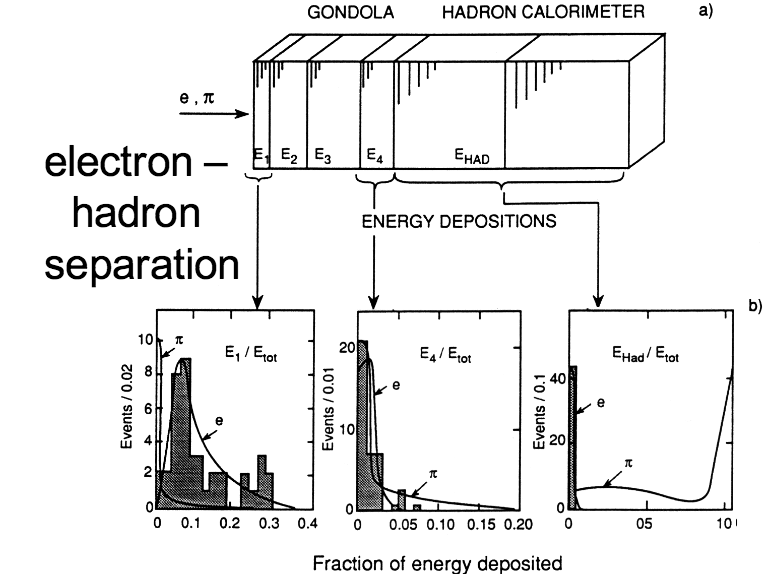
\includegraphics[height=0.6\textheight]{images/e-hadron-separation.png}
\end{figure}


\end{frame}

%------------------------------

\begin{frame}
\frametitle{Neutrino identification}
\fontsize{9pt}{12}\selectfont


\begin{itemize}
\item emission of neutrinos signalled via missing energy
\item calorimeters are completely hermetic down to $0.2^\circ$ in forward regions
\end{itemize}

\begin{figure}[h]
\centering
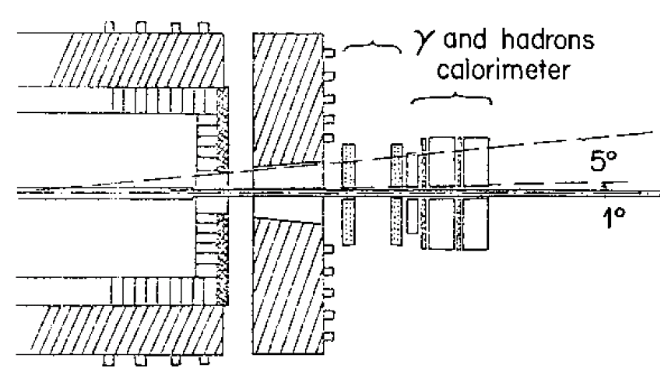
\includegraphics[height=0.6\textheight]{images/forward-region.png}
\end{figure}


\end{frame}

%------------------------------


\begin{frame}
\frametitle{Data taking}

\begin{itemize}
\item proton and anti-protons collided at $\sqrt{s}=\SI{540}{GeV}$
\item $\SI{18}{nb^{-1}}$ data set ($\sim 10^9$ collisions), collected at UA1
\item recorded over 30 days during November and December 1982
\item triggers were used to select events of interest
\end{itemize}


\end{frame}

%------------------------------

\begin{frame}
\frametitle{Triggers}
\fontsize{9pt}{12}\selectfont

\begin{itemize}
\item four initial event selections are performed:
\begin{enumerate}
\item[(1)] at least $\SI{10}{GeV}$ of $E_T$ in 2 gondolas or 2 bouchons
\end{enumerate}
\item with three other specific triggers for electron events:
\begin{enumerate}
\item[(2)] jet trigger: $\geq \SI{15}{GeV}$ of $E_T$ in localised EM/hadron calorimeter
\item[(3)] global $E_T$ trigger: $>\SI{40}{GeV}$ of total $E_T$; $|\eta|<1.4$
\item[(4)] muon trigger: at least one track with $|\eta|<1.3$
\end{enumerate}
\end{itemize}

\begin{itemize}
\item of $9.75\times 10^5$ events trigger, $1.4\times 10^5$ passed the above trigger selection, i.e. characterised by electron trigger flag
\end{itemize}


\end{frame}

%------------------------------

\begin{frame}
\frametitle{Offline selection}
\fontsize{11pt}{12}\selectfont

\begin{itemize}
\item number of events reduced to 27,000 after initial offline selection (using calorimeter)
\begin{itemize}
\item $E_T> \SI{15}{GeV}$ in two gondolas, or
\item $E_T > \SI{15}{GeV}$ in two bouchons with valid position information
\end{itemize}
\item again reduced with drift chamber reconstruction, requiring good quality, vertex-associated charged track of $p_T>\SI{7}{GeV/c}$
\begin{itemize}
\item 2,125 events remaining
\end{itemize}
\end{itemize}



\end{frame}

%------------------------------

\begin{frame}
\frametitle{Electron candidate selection}
\fontsize{12pt}{12}\selectfont

\begin{itemize}
\item from sample of 2,125 events, a final set of selections are applied to select for electrons
\item three cuts are made in succession to reduce jet debris
\begin{itemize}
\item 167 events remaining
\end{itemize}
\item two cuts are made to optimise selection for electromagnetic properties
\begin{itemize}
\item 39 events remaining
\end{itemize}
\end{itemize}


\end{frame}

%------------------------------

\begin{frame}
\frametitle{Electron candidate selection}
\fontsize{11pt}{12}\selectfont

\begin{itemize}
\item these 39 events are processed manually in Megatek and classified as:
\begin{enumerate}
\item[(1)] 5 events - jetless 
\item[(2)] 11 events - jet opposite track within $30^\circ$ angle of $\phi$
\item[(3)] 23 events - two jets (one containing electron candidate) or $e^+e^-$ conversion pair
\end{enumerate}
\item events with jets show no missing energy; jetless events show missing transverse energy almost exactly back-to-back to electron candidate
\end{itemize}


\end{frame}

%------------------------------

\begin{frame}
\frametitle{An aside - Megatek}
\fontsize{9pt}{12}\selectfont

\begin{figure}[h]
\centering
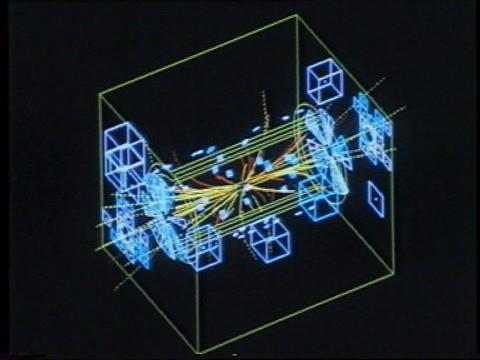
\includegraphics[height=0.6\textheight]{images/megatek.jpg}
\end{figure}

\begin{itemize}
\item Megatek examples (short movie) available at the \href{https://cds.cern.ch/record/1049887?ln=en}{CERN Document Server}
\end{itemize}

\end{frame}

%------------------------------



\begin{frame}
\frametitle{Electron candidate selection}
\fontsize{12pt}{12}\selectfont

\begin{columns}
\column{0.4\linewidth}

\begin{figure}[h]
\centering
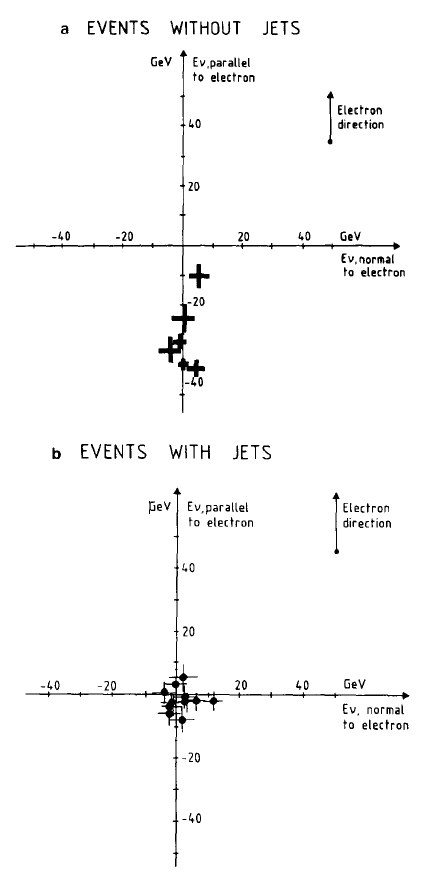
\includegraphics[height=0.85\textheight]{images/electron-selection-energy.png}
\end{figure}


\column{0.6\linewidth}

\begin{figure}[h]
\centering
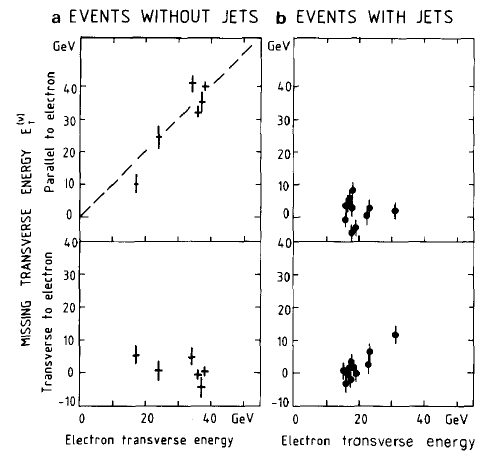
\includegraphics[width=0.9\textwidth]{images/electron-selection-transverse-energy.png}
\end{figure}


\end{columns}

\end{frame}

%------------------------------


\begin{frame}
\frametitle{Energetic neutrino candidate selection}
\fontsize{12pt}{12}\selectfont

\begin{itemize}
\item from sample of 2,125 events, a different set of selections are applied to search for energetic neutrinos
\item based exclusively on presence of missing $E_T$
\item two simple cuts are made to select high missing $E_T$ and candidate track not part of jet
\begin{itemize}
\item 70 events remaining
\end{itemize}
\item remaining events are processed manually, and two more cuts are applied
\begin{itemize}
\item 18 events remaining
\end{itemize}
\end{itemize}


\end{frame}

%------------------------------

\begin{frame}
\frametitle{Energetic neutrino candidate selection}
\fontsize{12pt}{12}\selectfont

\begin{columns}
\column{0.5\linewidth}

\begin{figure}[h]
\centering
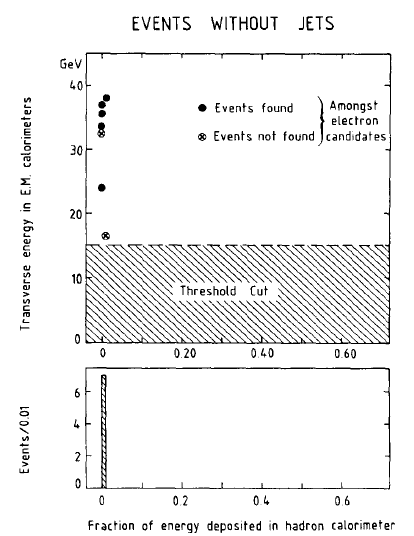
\includegraphics[width=0.85\textwidth]{images/neutrino-without-jets.png}
\end{figure}


\column{0.5\linewidth}

\begin{figure}[h]
\centering
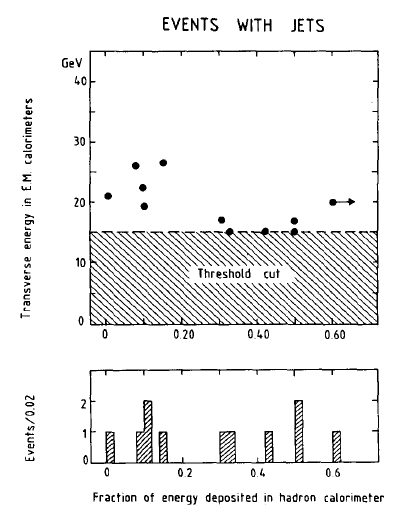
\includegraphics[width=0.85\textwidth]{images/neutrino-with-jets.png}
\end{figure}


\end{columns}

\end{frame}

%------------------------------

\begin{frame}
\frametitle{Energetic neutrino candidate selection}
\fontsize{12pt}{12}\selectfont

\begin{itemize}
\item from $E_c$ consideration, events with jets are deduced as hadronic events; the jetless events constitute an electron sample
\item five of the seven jetless events match the jetless events from electron candidate selection
\end{itemize}


\end{frame}

%------------------------------

\begin{frame}
\frametitle{Detailed event description}
\fontsize{12pt}{12}\selectfont

\begin{figure}[h]
\centering
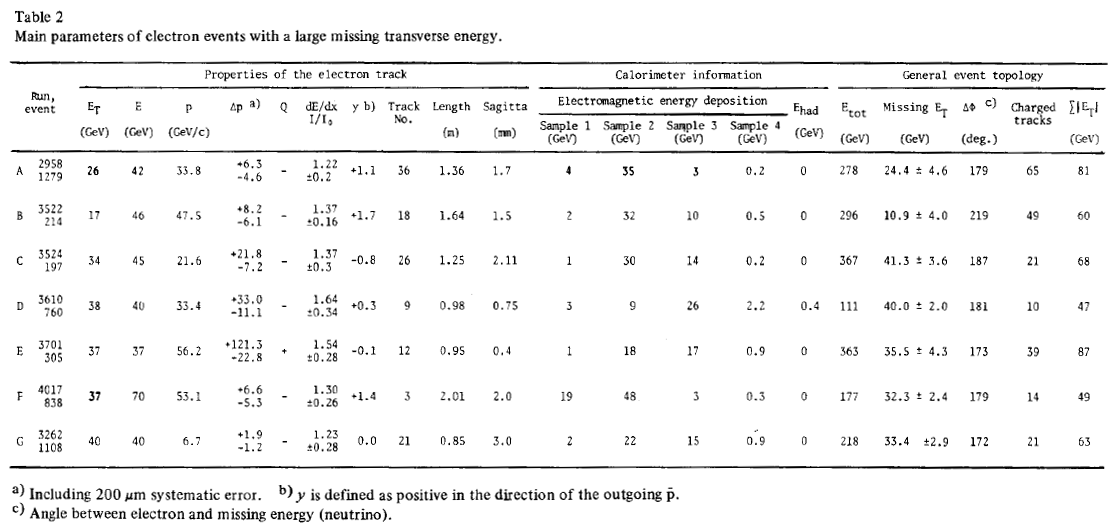
\includegraphics[width=\textwidth]{images/event-information.png}
\end{figure}


\end{frame}


%------------------------------

\begin{frame}
\frametitle{Background evaluations}
\fontsize{11pt}{12}\selectfont

\begin{itemize}
\item possible backgrounds:
\begin{enumerate}
\item[(1)] high $p_T$ $\pi^{\pm}$ misidentified as an electron or overlapping with one or more $\pi^0$
\item[(2)] high $p_T$ $\pi^0,\eta^0$ or $\gamma$ converted to $e^+ e^-$ pair with one side missed
\item[(3)] heavy quark production, with $Q_1\to e(\nu X)$ and $Q_2\to \nu(\ell X)$ and only the electron and neutrino being detected
\end{enumerate}
\item none of these background processes were shown to have occured; the final events are concluded to be high-energy electron events
\end{itemize}


\end{frame}

%------------------------------

\begin{frame}
\frametitle{A promising conclusion?}
\fontsize{12pt}{12}\selectfont

\begin{itemize}
\item presence of electron and neutrino of approximately equal and opposite transverse momenta suggests two body decay
\item[]
\item e.g. $W\to e+\nu_e$
\end{itemize}


\end{frame}

%------------------------------

\begin{frame}
\frametitle{Determining W mass}
\fontsize{10pt}{12}\selectfont

\begin{itemize}
\item lower limit on $m_W$ can be determined through $m_W\geq m_T$
\end{itemize}
\begin{equation*}
m_T^2=2p_T^{(e)}p_T^{(\nu)}(1-\cos\phi_{\nu e})
\end{equation*}
\begin{equation*}
m_W > \SI{73}{GeV/c^2} \text{at 90\% CL}
\end{equation*}
\begin{figure}[h]
\centering
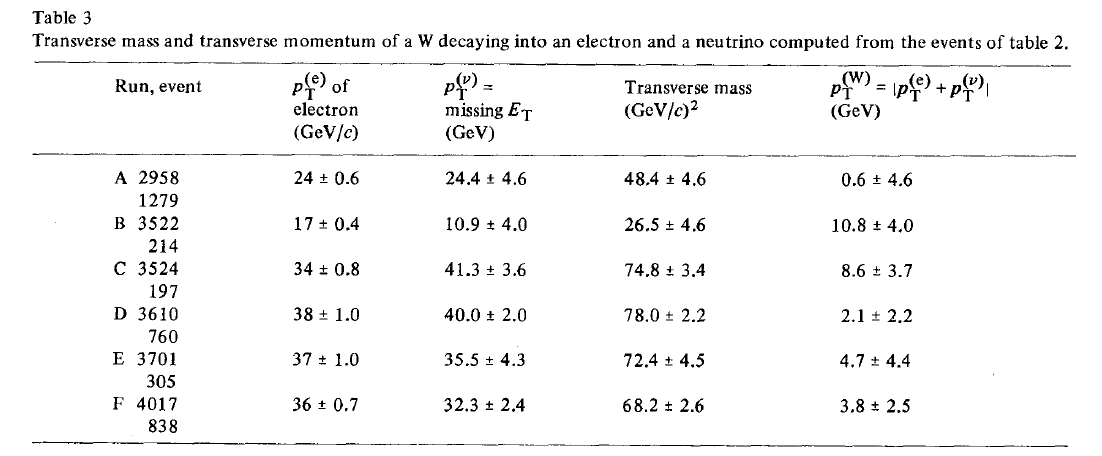
\includegraphics[width=0.8\textwidth]{images/transverse-mass.png}
\end{figure}


\end{frame}

%------------------------------


\begin{frame}
\frametitle{Determining W mass}
\fontsize{10pt}{12}\selectfont

\begin{itemize}
\item final fit corrects for transverse $W$ motion and uses Drell-Yan predictions with no smearing
\item mass given for fit on electron energy and angle and neutrino $E_T$ is
\end{itemize}

\begin{equation*}
m_W=\left(81^{+5}_{-5}\right)\text{GeV}/\text{c}^2
\end{equation*}

\begin{itemize}
\item excellent agreement with Weinberg-Salam model expected mass ($m_{W}=(82\pm 2.4)~\SI{}{GeV/c^2}$)
\item number of observed events (6) consistent with cross-section estimates ($\sim 7.2 k$)
\end{itemize}

\end{frame}

%------------------------------

\begin{frame}
\frametitle{End}

\begin{itemize}
\item Thank you for your attention
\item[]
\item Questions?
\end{itemize}

\end{frame}


%-------------------------------------------------------------------------------
%-------------------------------------------------------------------------------

 
\end{document}






